\documentclass[12pt]{article}

%Paquetes
\usepackage[left=2cm,right=2cm,top=3cm,bottom=3cm,letterpaper]{geometry}
\usepackage{lmodern}
\usepackage[T1]{fontenc}
\usepackage[utf8]{inputenc}
\usepackage[spanish,activeacute]{babel}
\usepackage{mathtools}
\usepackage{amssymb}
\usepackage{enumerate}
\usepackage{tabularx}
\usepackage{wasysym}
\usepackage{listings}
\usepackage{graphicx}
\usepackage{hyperref}
%\usepackage{graphicx}
%\graphicspath { {tarea01/media/} }
%\usepackage{pifont}
\usepackage{minted}
%Preambulo
\title{Tecnologías para desarrollos en internet \\ Manual CRUD: Beego}
\author{Kihui-DEV}
\date{Fecha: 18/09/16 \\ Facultad de Ciencias UNAM}

\begin{document}
\maketitle
\tableofcontents{}
\newpage

\section{Introducción}
Hola
\newpage
\section{Instalación de Go 1.7}
Paquetes de instalación para \textit{Apple OS X, Microsoft Windows y Linux} son provistos en la página oficial de descargas de \href{https://golang.org/dl/}{Go}. También viene incluido entre las opciones el código fuente del compilador del lenguaje junto con instrucciones para llegar a una instalación tan completa como las demás. \par
A continuación, presentamos la instalación para \textit{Linux y OS X}. \footnote{Si se desea revisar la configuración para \textit{Windows}, hacer uso del siguiente enlace:
  \href{https://golang.org/doc/install?download=go1.7.1.windows-amd64.msi}{MSI Installer}}

\subsection{Descarga}\label{sec:d}


\subsubsection*{Linux}
Para obtener el paquete de Golang\footnote{Actualmente la versión 1.7.1} \\
Ejecutar:
\begin{verbatim}
  $ wget https://golang.org/doc/install?download=go1.7.1.linux-amd64.tar.gz
\end{verbatim}
O bien descargarlo directamente desde este enlace:
\begin{center}
\href{https://golang.org/doc/install?download=go1.7.1.linux-amd64.tar.gz}{Go 1.7 para Linux y OS X}.
\end{center}


\subsubsection*{Mac OS X}
Alternativa a las siguientes instrucciones, existe la opción de descargar el fichero \textit{.pkg} instalable de \textit{Go} que automatiza la configuración para este sistema operativo.\footnote{\href{https://golang.org/doc/install?download=go1.7.1.darwin-amd64.pkg}{Instalador para Mac OS X}}\\[1mm]

Para obtener una configuración inicial personalizada \textit{Mac OS X} utilice el paquete descargable para \textit{Linux} disponible en la sección anterior.\\

El resto de la configuración se sigue de la misma manera para ambas plataformas.

\subsection{Configuración}\label{sec:c}
Primero extraemos los archivos del paquete comprimido sobre algún directorio.\\
Para descomprimir el paquete sobre \textit{/usr/local} como es usual:
\begin{verbatim}
  # tar -C /usr/local -xzf go1.7.1.linux-amd64.tar.gz
\end{verbatim}
Al finalizar la extracción, procedemos a establecer una ruta a los binarios de las herramientas de \textit{Go}, y así tenerlas disponibles en cada sesión.\par
Agregar esta línea en el script de inicio (típicamente sobre \textit{/user/local/profile}
si se desea hacer una instalación general en el sistema operativo o
en particular para el usuario en curso, usar en cambio \textit{\char126/.profile}):
\begin{verbatim}
  export PATH=$PATH:/usr/local/go/bin
\end{verbatim}

\subsection{Prueba}
Crear un directorio que haga de workspace para la prueba.\\
Por ejemplo:
\begin{verbatim}
  $ mkdir ~/go
\end{verbatim}
Asignar la variable \textbf{GOPATH}\footnote{La misma línea puede agregarse al script de inicio \textit{profile} manejado en la sección de configuracion para evitar ejecutarla y mantener los proyectos y aplicaciones de \textit{Go} ubicados en un sólo directorio.}
para que apunte a tal dirección:
\begin{verbatim}
  $ export GOPATH=$HOME/go
\end{verbatim}
Bien podemos hacer persistente este cambio agregando la misma línea al script
de inicio que editamos en la sección anterior (ir a Descarga~\ref{sec:d} y configuración~\ref{sec:c}). \par

A continuación, creamos dentro de ese directorio  \textit{src/hola}.
Y dentro de \textit{hola/} un fichero nuevo de nombre \textit{hola.go}:
\begin{verbatim}
     package main

     import "fmt"

     func main() {
         fmt.Printf("hola, mundo\n")
     }
\end{verbatim}

Luego, desde cualquier ubicación podemos ejecutar\\
esto:
\begin{verbatim}
  $ go install hola
\end{verbatim}

Esto producirá un ejecutable \textit{hola} dentro de el directorio \textit{go/bin/},
que podemos ejecutar utilizando lo siguiente:
\begin{verbatim}
  $ $GOPATH/bin/hola
\end{verbatim}

o directamente sobre el directorio donde se encuentre el ejecutable:

\begin{verbatim}
  $ ./hola
\end{verbatim}

Si produce la salida ``hola, mundo'', quiere decir que nuestra instalación fue exitosa. \newpage


\section{Instalación de Beego}

\noindent Para instalar la última versión de Beego\footnote{A la fecha de elaboración de este manual: 1.7.1} utilizamos el siguiente comando:
\begin{verbatim}
  $ go get github.com/astaxie/beego
\end{verbatim}

\noindent Para compilar y correr nuestros proyectos necesitaremos instalar Bee\footnote{A la fecha de elaboración de este manual: 1.5.2} también :
\begin{verbatim}
  $ go get github.com/beego/bee
  $ go install github.com/beego/bee
\end{verbatim}

Para poder utilizar \textit{bee} sin necesidad de ir a la carpeta de binarios de \textit{Go}, podemos crear un enlace simbólico que apunte precisamente al ejecutable.
\begin{verbatim}
  # ln -s $GOPATH/bin/bee /usr/bin/bee
\end{verbatim}

\section{Creación de proyecto}\label{sec:proy}
\noindent Para crear un proyecto en Beego, necesitamos ir al directorio de nuestro $\$$GOPATH, donde escribimos el siguiente comando:
\begin{verbatim}
$ bee new beego-crud
\end{verbatim}
\noindent Podremos ver que se han creado las siguientes carpetas y archivos necesarios para nuestra aplicación:

\begin{verbatim}
beego-crud/
|-- conf/
|   |__ app.conf
|-- controllers/
|   |__ default.go
|-- main.go
|-- models/
|-- routers/
|   |__ router.go
|-- static/
|   |--- css/
|   |--- img/
|   |___ js/
|-- tests/
|   |__ default_test.go
|-- views/
    |__ index.tpl
\end{verbatim}

\subsection{Estructura del proyecto - MVC}
\begin{enumerate}[1)]
  \subsubsection*{Modelo}
\item \textit{conf/}
\item \textit{models/}
  \subsubsection*{Vista}
\item \textit{views/}
  \subsubsection*{Controlador}
\item \textit{controllers/}
\item \textit{routers/}
  \subsubsection*{Extra}
\item \textit{static/}
\item \textit{tests/}

\end{enumerate}


\subsection{Prueba del servidor local}\label{sec:pr}
\noindent Finalmente para correr el nuevo proyecto que hemos creado, hacemos lo siguiente:
\begin{verbatim}
$ cd $GOPATH/src/beego-crud
$ bee run
\end{verbatim}
\noindent Ingresamos \textit{localhost:8080} como dirección en el navegador para encontrarnos con la siguiente página de inicio: \\

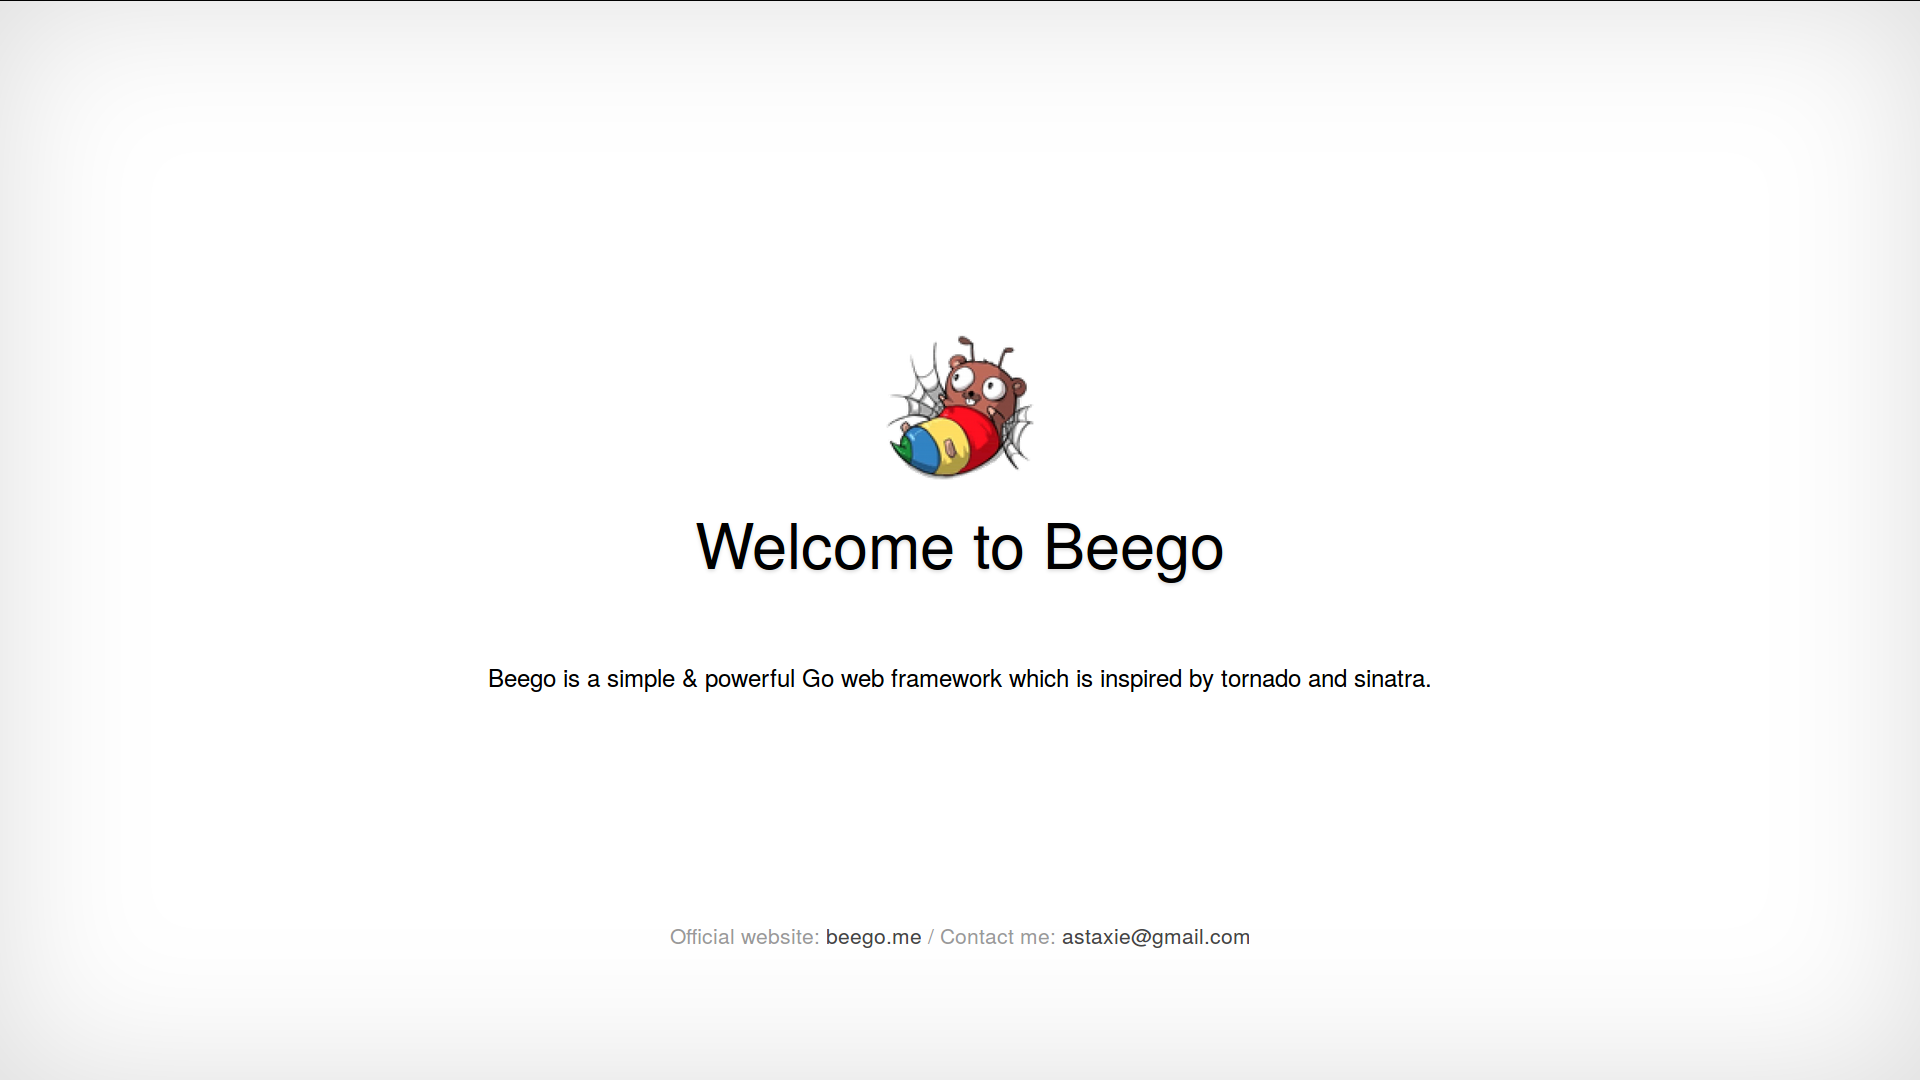
\includegraphics[scale=0.25]{beego.png}
\newpage

\section{Elaboración del CRUD bajo MVC}
En esta sección revisaremos la implementación de un CRUD (\textit{Create-Read-Update-Delete}) sobre la aplicación que creamos en la sección anterior (s.~\ref{sec:proy}). Comenzaremos explicando los documentos que tenemos que modificar para tener una configuración exitosa y la forma de escribir el código de acuerdo al MVC (\textit{Modelo Vista Controlador}), siguiendo la estructura que nos proporciona \textit{Beego} para éste.

\subsection{Preparación}
%Para implementar nuestro primer CRUD en Beego es necesario tener un sistema de
%datos persistente sobre el
%que realicemos nuestras operaciones.
%La mejor solución que en casi todos los casos se señala para lograr esto en el desarrollo
%web por supuesto no son los archivos, sino una base de datos, por lo general
%relacional. \par
Todo proyecto de Beego, como ya vimos, está organizado segun el MVC. Es precisamente
sobre el archivo de \textbf{models.go} que escribiremos nuestras
relaciones expresadas con atributos asignados de acuerdo a los tipos de dato
que maneja Go para después verlos reflejados en tablas en una base datos ya explorable.
Bien podría ser en sentido inverso, desde un esquema \textit{SQL} generar los modelos
para nuestro proyecto de Beego, pero en nuestro caso decidimos implementarlo
en esta dirección porque nuestra intención es enfocarnos en Beego, no en SQL.\par
A continuación presentamos la configuración de la base de datos y un mapeo
de una sola relación con la que trabajaremos todas las operaciones.
\subsubsection*{Base de datos}
\textit{Beego-ORM} es la herramienta de Mapeo Objeto-Relacional de \textit{Beego}
escrita en \textit{Go}. Según la página oficial está inspirada en \textit{Django ORM}
y \textit{SQLAlchemy}. Se advierte que al estar en desarrollo, no se garantiza
un 100\% de compatibilidad y es posible encontrar algunos ``bugs'', que el
equipo de desarrollo de Beego promete solucionar apenas se reporten.\\

Lo primero que hay que considerar es la conexión con la base de datos que necesitamos para nuestro modelo.
Beego provee soporte para tres sistemas manejadores de bases de datos
con sus respectivos ``drivers'':
\begin{itemize}
\item \href{http://www.mysql.com/}{MySQL}
\item \href{https://sqlite.org/}{Sqlite}
\item \href{http://www.postgresql.org.es/}{Postgres}
\end{itemize}

Por su sencilla configuración y mayoría de ejemplos de implementación junto con
Beego, escogimos MySQL por lo que los siguientes puntos se ejemplificarán
con el supuesto de que trabajamos con este SMBD\footnote{Para revisar más ampliamente
  las opciones de bases de datos recomendamos visitar este apartado de la documentación:
  \href{http://beego.me/docs/mvc/model/orm.md\#set-up-database}{ORM Usage}} y que ya se cuenta con una instalación
funcional\footnote{En el manual de MySQL v5.7 viene una amplia guía de instalación.
  Recomendamos los siguientes apartados para distintos sistemas operativos:
  \href{http://dev.mysql.com/doc/refman/5.7/en/windows-installation.html}{Windows} |
  \href{http://dev.mysql.com/doc/refman/5.7/en/osx-installation.html}{OS X} |
  \href{http://dev.mysql.com/doc/refman/5.7/en/linux-installation.html}{Linux}}.\\[2mm]
Lo primero que haremos será crear nuestra base de datos:
\begin{verbatim}
  $ mysql -u root -p
  MariaDB [(none)]> create database beego;
  MariaDB [(none)]> exit
\end{verbatim}
Si no experimentamos ninguna dificultad con esto, podemos continuar con la
configuración de nuestro proyecto.
\subsubsection*{Configuración}
Todo proyecto de \textit{Beego} cuenta con un archivo de configuración.
Por defecto se interpreta el archivo \textbf{app.conf} bajo el directorio
\textit{conf/} de la aplicación. Inicialmente, dicho archivo está escrito en formato INI
\footnote{También se permiten los siguientes formatos: XML, JSON y YAML},
una sintáxis sencilla, compuesta de
secciones, propiedades y valores sobre archivos de texto plano. Por ejemplo, en ella podremos escribir
configuraciones del estilo:
\begin{verbatim}
  [seccion]
  nombre_propiedad = valor
\end{verbatim}

Nosotros conservaremos el nombre de la aplicación (appname), el puerto http
(httport) y el modo de ejecución (runmode); propiedades que ya vienen incluídas
al momento de creación de nuestra nueva aplicación. Adicionalmente
escribiremos las siguientes propiedades:\footnote{El caracter ``;'' denota una línea de comentario. No es necesario
  al final de cada línea. }
\begin{verbatim}
  mysqluser = "root" ;el nombre del usuario de MySQL que es dueño de la base
  mysqlpass = "magdario" ;la contraseña de acceso del usuario MySQL
  mysqldb = "beego" ;el nombre de la base de datos que creamos anteriormente
  mysqlurls = "127.0.0.1" ;la dirección del host de la base de datos (localhost)
\end{verbatim}

Gracias a esta configuración la aplicación podrá establecer
conexión con nuestra base de datos para llevar a cabo las operaciones.

\subsubsection*{Modelos}\label{sec:p}
Como ya señalamos previamente, para realizar el CRUD, nos auxiliaremos de una
sola relación en la base de datos.
Para registrarla, basta definir una estructura
sobre el archivo de Go \textbf{models.go}, ubicado en la carpeta \textit{models/}
de nuestra aplicación. Aquí mostramos un ejemplo de cómo podría ser un modelo de
usuario\footnote{Para revisar con más detenimiento el código, pruebe visualizar
  el archivo del proyecto en GitHub: \href{https://github.com/Kihui/Beego-CRUD/blob/master/models/models.go}{models.go}}:

\begin{minted}{go}
  type Usuario struct {
      Id          int
      Nombre      string
      Edad        int
  }
\end{minted}

Para continuar con el mapeo y ver nuestro nuevo modelo reflejado en la base
de datos que configuramos previamente,
ahora nos dirigimos al archivo \textbf{main.go} en la raíz del proyecto y
agregamos las siguientes configuraciones a los ``imports'' del programa:
\begin{minted}{go}
    "github.com/astaxie/beego/orm"
    _ "github.com/go-sql-driver/mysql"
    models "beego-crud/models"
\end{minted}
Esto con el fin de que podamos utilizar Beego-ORM, el driver del SMBD
y los modelos que declaremos. \\
Luego, creamos un nuevo método método \textit{init()}, en el que escribiremos:
\begin{minted}{go}
    func init() {
        orm.RegisterDriver("mysql", orm.DRMySQL)
        orm.RegisterDataBase("default", "mysql", "root:magdario@/beego?charset=utf8")
        orm.RegisterModel(new(models.Usuario))
        orm.RunCommand()
    }
\end{minted}

Con esto, registramos tanto el driver que utilizaremos como la base de datos sobre
la que se realizaran las operaciones de los modelos que ``demos de alta''
en este método. Es importante señalar que si no registramos los modelos aquí o
en su archivo correspondiente, no serán ``visibles'' para nuestra aplicación y no
será posible efectuar cambios sobre ellos. Nosotros elegimos registrar el modelo
de \textit{usuario}  en el método de inicialización, por la forma explícita que nos provee. \\

\noindent
Recomendamos revisar la forma resultante del archivo: \href{https://github.com/Kihui/Beego-CRUD/blob/master/main.go}{main.go} \\

Finalmente, compilamos \textbf{main.go} y lo ejecutamos con los parámetros necesarios
para realizar el mapeo y la sincronización con la base de datos.\\

\noindent
Desde \textit{\$GOPATH/beego-crud} ejecutamos:
\begin{verbatim}
  $ go build main.go
  $ ./main orm syncdb
\end{verbatim}

\noindent
Para revisar que todo marcha bien podemos pedirle al ``prompt'' de MySQL que nos
muestre las tablas de nuestra base de datos:
\begin{verbatim}
  MariaDB [(none)]> use beego;
  MariaDB [beego]> show tables;
\end{verbatim}

\noindent
Que debe resultarnos en algo similar a:
\begin{verbatim}
+-----------------+
| Tables_in_beego |
+-----------------+
| usuario         |
+-----------------+
\end{verbatim}

Si en efecto nos encontramos con las tablas correspondientes a los modelos que
registramos, ya podemos dedicarnos a escribir el controlador y las vistas
pertinentes para nuestro CRUD, sin preocuparnos por la conexión con la base
de datos.\\

A continuación presentamos las operaciones de un CRUD implementado en nuestro
Framework Beego. Cada una viene separada con su sección correspondiente y los
apartados que contiene se refieren a los archivos de la estructura del proyecto
y cómo debemos modificarlos para elaborar la operación en cuestión.\\

\subsection{Creación}
Manejaremos esta operación como un registro de usuarios para alguna plataforma.
Este registro será lo primero que tendremos en el ``index'' de la página que
estamos desarrollando.
\subsubsection{Controllers}
Lo primero que debemos considerar es la función del controlador que manejara
nuestra operación de creación. En el archivo controllers/\textbf{default.go}\footnote{Podemos cambiar este nombre de archivo si nos parece pertinente, pero por simplicidad lo dejaremos así, basta con que nuestras funciones de controlador se ubiquen en esa carpeta.}
encontraremos la estructura del controlador principal, sus métodos serán los que
manejen las respuestas del servidor ante las peticiones de la interfaz.
Antes de comenzar con nuestra función de agregado o creación de usuario, importaremos
los modelos de la aplicación que ya hemos considerado\footnote{Preparación - Modelos \ref{sec:p}},
la herramienta \textit{ORM} (mapeo y conexión con la base de datos), una herramienta de validación
de datos y la herramienta estándar de Go \textit{fmt}:
\label{sec:imp}
\begin{minted}{go}
    import (
      "github.com/astaxie/beego"
      models "beego-crud/models"
      "github.com/astaxie/beego/orm"
      "github.com/astaxie/beego/validation"
      "fmt"
    )
\end{minted}
Posteriormente, crearemos efectivamente nuestra función de agregado, que
llamaremos \textit{Add()}. Prestemos particular atención a la estructura (recordemos
que Go, como C, es un lenguaje estructurado) llamada MainController.
\begin{minted}{go}
  // Método que permite registrar un nuevo usuario
  func (this *MainController) Add() {
    this.TplName = "index.tpl"
    o := orm.NewOrm()
    o.Using("default")

    // Se crea un nuevo usuario
    u := models.Usuario{}
    // Se guardan los datos del formulario en el nuevo usuario
    if err := this.ParseForm(&u); err != nil {
      // Si hay errores en el formulario
      beego.Error("Error: ", err)
    } else {
      this.Data["Usuarios"] = u
      // Se validan los datos del usuario
      valid := validation.Validation{}
      isValid, _ := valid.Valid(u)
      if !isValid {
        this.Data["Errors"] = valid.ErrorsMap
        beego.Error("Datos inválidos")
      } else {
        // Se inserta el usuario nuevo en la base de datos
        id, err := o.Insert(&u)
        if err == nil {
          msg := fmt.Sprintf("Nuevo usuario con id: ", id)
          beego.Debug(msg)
        } else {
          msg := fmt.Sprintf("No se pudo registrar usuario: ", err)
          beego.Debug(msg)
        }
      }
    }

    var usuarios []*models.Usuario
    num, err := o.QueryTable("usuario").All(&usuarios)

    if err != orm.ErrNoRows && num > 0 {
      this.Data["records"] = usuarios
    }
  }
\end{minted}
Veamos que una de las primeras instrucciones que se dan es definir un template
para la función de agregado del controlador, ello lo consideraremos más adelante (sección \ref{sec:unov}).
A continuación, agregaremos una configuración en los \textit{routers} para poder
hacer uso de nuestra nueva función.
\subsubsection{Routers}
Como ya hemos señalado anteriormente, el archivo de las rutas o ``urls'' de nuestra
aplicación web, se encuentra bajo el directorio \textit{routers/} con el nombre de
\textbf{router.go}. En él nos encontraremos con una ruta por defecto, esta es la que
nos muestra apenas visitamos el servidor de \textit{Bee} luego de crear nuestra
nueva aplicación (sección \ref{sec:pr}).
\begin{minted}{go}
  beego.Router("/", &controllers.MainController{})
\end{minted}
Ahora, modificaremos esa línea para que sea acorde a nuestra operación de creación.
\begin{minted}{go}
  beego.Router("/", &controllers.MainController{}, "post:Add")
\end{minted}
Y listo, nuestra aplicación llamará a la función de agregado en cuanto se haga
una petición al servidor por esa ruta.
\subsubsection{Views}\label{sec:unov}
Con el fin de que nuestra ruta previamente creada funcione, debemos crear un
archivo \textit{.tpl} que corresponda con la plantilla (template) que indicamos
en la función del controlador que llama la ruta del servidor. En este caso la ruta
\textit{localhost:8080/}, y la función \textbf{Add()}. \\

Toda plantilla debe ubicarse bajo el directorio \textit{views/} de la aplicación.
Básicamente, consisten de un documento HTML con anotaciones propias del framework
que hacen referencia a estructuras que maneja el controlador.
Nosotros indicamos el template de la función de agregado como \textbf{index.tpl},
por lo que crearemos la plantilla correspondiente con dicho nombre.
Esta parte la dejaremos a su consideración\footnote{Es posible encontrar nuestro
  template funcional con \textit{MaterialDesign} como framework de frontend
  \href{https://github.com/Kihui/Beego-CRUD/blob/master/views/index.tpl}{aquí}.\\
  Es importante recordar que la aplicación de Beego cuenta con un directorio \textit{static/}
para manejar los estilos de los templates.},
por la cuestión del estilo,
sin embargo, les dejamos un ejemplo en HTML\footnote{Nótese que el pattern del correo
  electrónico no está definido, por lo que recomendamos dirigirse al FINAL de la siguiente
  sección del documento para conocer las razones: \ref{regexp}}
sin estilo para guiarlos en el proceso de elaboración:
\begin{minted}{html}
 <!DOCTYPE html>
  <html>
  <head>
    <title>Beego-CRUD</title>
    <meta http-equiv="Content-Type" content="text/html; charset=utf-8">
  </head>

  <body>
    <h3 class="beego">CRUD de Beego</h3>
    <h4>Agregar Usuario</h4>
    <form role="form" id="usuario" method="POST">
      <div class="">
        <input id="nombre" name="nombre" value="{{.Usuario.Nombre}}" type="text" />
        <label for="nombre">Nombre</label>
      </div>
      <br/>
      <div>
        <input id="app" name="app" value="{{.Usuario.App}}" type="text" />
        <label for="app">Apellido Paterno</label>
      </div>
      <br/>
      <div class="">
        <input id="apm" name="apm" value="{{.Usuario.Apm}}" type="text" />
        <label for="apm">Apellido Materno</label>
      </div>
      <br/>
      <div class="">
        <input id="correo" name="correo" pattern="" value="{{.Usuario.Correo}}" type="text" />
        <label for="correo">Correo Electrónico</label>
      </div>
      <br/>
      <div class="">
        <input id="edad" pattern="[0-9]*?" name="edad" value="{{.Usuario.Edad}}" type="text" />
        <label for="edad">Edad</label>
      </div>
      <br/>
      <input type="submit" value="Aceptar" />
    </form>
  </div>
</body>
</html>

\end{minted}
\subsection{Lectura}
Esta operación será implementada para la página principal de nuestro CRUD,
junto con la operación de creación. Esto con el fin de que sea observable
que ambas operaciones funcionan sin necesidad de hacer consultas en la base de
datos. Como tal, el usuario no tendrá interacción con esta operación, eventualmente
será ``modificable'', o mejor dicho observable (en los cambios) con las
operaciones restantes.\\

A continuación, se presenta la misma lógica para la operación
de creación previa.
\subsubsection{Controllers}
Para este punto suponemos que ya se han expresado las importaciones (\ref{sec:imp})
necesarias en el archivo de \textit{default.go} que tiene nuestro controlador
principal. Continuaremos con la elaboración del método que manejará la lectura
o consulta de los usuarios en la base de datos que llamaremos \textbf{View()}:

\begin{minted}{go}
  // Método que muestra todos los usuarios
  func (c *MainController) View() {
    // Nombre del template
    c.TplName = "index.tpl"
    // Se le asigna un modelo al formulario de la vista
    c.Data["Form"] = &models.Usuario{}
    // Se crea una conexión a la base
    o := orm.NewOrm()
    // Se indica que se usará la base por default
    o.Using("default")

    // Arreglo donde se guardarán los usuarios
    var usuarios []*models.Usuario
    // Se guardan los usuarios de la base en el arreglo
    num, err := o.QueryTable("usuario").All(&usuarios)

    if err != orm.ErrNoRows && num > 0 {
      // Se pasa el arreglo al contexto de la vista
      c.Data["records"] = usuarios
    }
  }
\end{minted}
Como se había mencionado, la funcionalidad de este método será observable desde la página
principal, es por eso que asignamos el mismo template que para la operación de creación
anterior. Es importante que tengamos presente el nombre de nuestra función, pues la
utilizaremos en el siguiente apartado. 
\subsubsection{Routers}
Con el fin de hacer disponible nuestra función, es debido incluirla en alguna de las
rutas de la aplicación. Modificando el archivo \textbf{routers.go} podemos asignar una
función a una o más rutas. Dado que esperamos que nuestra operación de lectura esté disponible
desde la página principal al igual que nuestra operación de creación, simplemente modificaremos
la línea que habíamos agregado previamente para incluír nuestra nueva operación de lectura.
Por tanto, de tener está línea:
\begin{verbatim}
  beego.Router("/", &controllers.MainController{}, "post:Add")
\end{verbatim}

\noindent Agregaremos la función \textbf{View()} de la siguiente manera:
\begin{minted}{go}
  beego.Router("/", &controllers.MainController{}, "get:View;post:Add")
\end{minted}
Finalmente, para poder probar nuestra nueva configuración será necesario editar el template de la página principal.
\subsubsection{Views}
El template que elegimos para la función de lectura, referente al archivo \textbf{index.tpl}
del directorio de vistas de la aplicación, ya debe existir si hemos implementado la operación
de creación del CRUD previamente. Simplemente agregaremos un contenedor pertinente para mostrar
la información del modelo que nos devuelve nuestra función recién realizada:
\begin{minted}{html}
    <div>
    <h4>Usuarios</h4>
    <table>
      <thead>
        <tr>
          <th>Nombre</th>
          <th>Correo</th>
          <th>Edad</th>
          <th></th>
          <th></th>
        </tr>
      </thead>
      <tbody>
        {{range $record := .records}}
        <tr>
          <td>{{$record.Nombre}} {{$record.App}} {{$record.Apm}}</td>
          <td>{{$record.Correo}}</td>
          <td>{{$record.Edad}}</td>
        </tr>
        {{end}}
      </tbody>
    </table>
  </div>
\end{minted}
Con estos cambios será posible visualizar los nuevos usuarios apenas los agreguemos sin necesidad
de cambiar de página. Todo desde la ruta principal de la aplicación \textit{localhost:8080/}.
\subsection{Actualización}
Supondremos que ya se ha implementado la operación de lectura como se describe en este documento
y que ya contamos con registros existentes de usuarios en la base de datos.
Continuaremos con la descripción de los pasos en la lógica de la aplicación; los mismos
seguidos en el desarrollo de las demás operaciones del CRUD.
\subsubsection{Controllers}
Como ya deben sospechar, luego de haber repetido los pasos dos veces con las operaciones anteriores,
lo primero será escribir una función en el archivo de controlador principal \textbf{routers.go}.
Por motivos de simplicidad, el nombre ideal nos parece ser \textbf{Update()}, pero es preciso
repetir que el nombre no afectará su funcionamiento, siempre que lo respetemos para las implementaciones
de los apartados siguientes. De lo contrario, podríamos confundir un simple error de referencia con uno
inmerso en la lógica de nuestra aplicación.
A continuación nuestra propuesta de código para el método de actualización:
\begin{minted}{go}
  // Método que permite modificar los datos de un usuario
  func (this *MainController) Update() {
    this.TplName = "update.tpl"
    this.Data["Form"] = &models.Usuario{}
    o := orm.NewOrm()
    o.Using("default")

    // Se obtiene el parámetro id del url
    if id, err := this.GetInt("id"); err == nil {
      // Se obtiene el usuario con el id del parámetro
      u := models.Usuario{Id: id}
      if o.Read(&u) != nil {
        beego.Error("El usuario no existe")
      } else {
        // Se pasan los datos del usuario al contexto de la vista
        this.Data["Nom"] = u.Nombre
        this.Data["App"] = u.App
        this.Data["Apm"] = u.Apm
        this.Data["Correo"] = u.Correo
        this.Data["Edad"] = u.Edad
      }
      // Si se efectúa el método POST en la vista
      if this.Ctx.Input.Method() == "POST" {
        // Se guardan los datos del formulario en el usuario
        if err := this.ParseForm(&u); err != nil {
          beego.Error("Error: ", err)
        } else {
          this.Data["Usuarios"] = u
          valid := validation.Validation{}
          isValid, _ := valid.Valid(u)
          if !isValid {
            this.Data["Errors"] = valid.ErrorsMap
            beego.Error("Datos inválidos")
          } else {
            // Se actualiza el usuario con los nuevos datos en la base
            id, err := o.Update(&u)
            if err == nil {
              msg := fmt.Sprintf("Usuario actualizado: ", id)
              beego.Debug(msg)
            } else {
              msg := fmt.Sprintf("No se pudo actulizar usuario: ", err)
              beego.Debug(msg)
            }
          }
        }			
        this.Redirect("/", 302)
        return
      }
    } else {
      beego.Error("Parámetro inválido: ", err)
    }		
  }
  
\end{minted}
Con este método listo, podemos proceder a configurarlo en las rutas de la aplicación y dejarlo
disponible.
A propósito de hacer más explícita la contraparte visual que le corresponde, hemos asignado el template de
esta función con el mismo nombre: \textbf{update.tpl}; archivo que deberá existir en el directorio de
vistas de la aplicación.
\subsubsection{Routers}
Anteriormente agregamos y, posteriormente modificamos, una sola ruta de la aplicación en la función
\textbf{init()} de nuestro archivo de configuración de rutas \textbf{router.go}.
Justo debajo (o arriba) de la línea que define la ruta principal de la aplicación, colocaremos
una que corresponda a la función de actualización recién presentada.
\begin{minted}{go}
  beego.Router("/update", &controllers.MainController{}, "*:Update")  
\end{minted}
Apreciemos que difiere en argumentos con la línea de la ruta principal. El primero nos indica que esta
funcionalidad es accesible desde \textit{localhost:8080/update}, sin embargo, para que el usuario
pueda hacer uso de la función adecuadamente no es conveniente que acceda de forma ``manual'' a dicha ruta de a aplicación,
pues necesitamos información de entrada, el usuario que será modificado -en nuestro caso, el id de dicho
elemento. 
\subsubsection{Views}
Con la intención de resolver la situación planteada al final del apartado anterior,
alteraremos un poco la vista principal de la aplicación para hacer posible la
modificación de usuarios existentes en la base de datos.
Añadiremos una línea en la vista principal \textbf{index.tpl} (dentro de la definición de
la tabla).
\begin{verbatim}
  <tr>
    <td>{{$record.Nombre}} {{$record.App}} {{$record.Apm}}</td>
    <td>{{$record.Correo}}</td>
    <td>{{$record.Edad}}</td>
  </tr>
\end{verbatim}
Resultando en lo siguiente:
\begin{minted}{html}
  <tr>
    <td>{{$record.Nombre}} {{$record.App}} {{$record.Apm}}</td>
    <td>{{$record.Correo}}</td>
    <td>{{$record.Edad}}</td>
    <td><a href="/update?id={{$record.Id}}"><i>editar</i></a></td>
  </tr>
\end{minted}
Posteriormente, ya que hemos hecho accesible la ruta de la operación de actualización
con el parámetro necesario para la función del controlador que le corresponde, 
obligatoriamente debemos incluir el template que exige en el directorio de vistas.\\
\textit{views/}\textbf{update.tpl}:
\begin{minted}{html}
  <!DOCTYPE html>
   <html>
   <head>
    <title>Beego-CRUD</title>
    <meta http-equiv="Content-Type" content="text/html; charset=utf-8"/>
   </head>

   <body>
    <div>
      <h3 class="beego">CRUD de Beego</h3>
      <h4>Actualizar Usuario</h4>
      <form role="form" id="usuario" method="POST">
       <div>
         <input id="nombre" name="nombre" value="{{.Nom}}" type="text" />
         <label for="nombre">Nombre</label>
       </div>
       <br/>
       <div>
         <input id="app" name="app" value="{{.App}}" type="text" />
         <label for="app">Apellido Paterno</label>
       </div>
       <br/>
       <div>
         <input id="apm" name="apm" value="{{.Apm}}" type="text" />
         <label for="apm">Apellido Materno</label>
       </div>
       <br/>
       <div>
         <input id="correo"  name="correo" pattern="" value="{{.Correo}}" type="text" />
         <label for="correo">Correo Electrónico</label>
       </div>
       <br/>
       <div>
         <input id="edad" pattern="[0-9]*?" name="edad" value="{{.Edad}}" type="text" />
         <label for="edad">Edad</label>
       </div>
       <br/>
       <input type="submit" value="Aceptar" /> 
      </form>
    </div>
  </body>
 </html>  
\end{minted}
\label{regexp}
No pasemos por alto que el patrón del correo debe ser llenado con una expresión regular.
Por limitantes en el ancho de página, no pudimos agregar nuestro original al HTML
que presentamos. Pero he aquí el que nosotros utilizamos:
\begin{verbatim}
[a-z0-9._%+-]+@[a-z0-9.-]+\.[a-z]{2,4}$
\end{verbatim}
\subsection{Eliminación}
Para terminar con la implementación de nuestro CRUD en Beego, implementaremos
la eliminación de usuarios. De manera similar a la operación de actualización
anterior, estará disponible la función de eliminación en el listado de lectura
de usuarios de la página principal. A un lado de la edición de un usuario en la
tabla, tendremos la opción de eliminarlos.
\subsubsection{Controllers}
Dentro del archivo del controlador principal \textit{controllers/}\textbf{default.go}
crearemos una nueva función de eliminación para la estructura que ahí reside.
Le llamaremos de forma convencional con el nombre \textbf{Delete()}.
Aquí su implementación:
\begin{minted}{go}
  // Método que permite eliminar un usuario
  func (this *MainController) Delete() {
    this.TplName = "delete.tpl"
    // Se obtiene el parámetro id del url
    id, err := this.GetInt("id")
    if err != nil {
      msg := fmt.Sprintf("Parámetro inválido: ", err)
      beego.Debug(msg)
    }

    o := orm.NewOrm()
    o.Using("default")

    // Se obtiene el usuario con el id del parámetro
    if existe := o.QueryTable("usuario").Filter("Id", id).Exist(); existe {
      // Se elimina el usuario de la base de datos
      if num, err := o.Delete(&models.Usuario{Id: id}); err == nil {
        beego.Info("Usuario eliminado. ", num)
      } else {
        beego.Error("Usuario no pudo ser eliminado: ", err)
      }
    } else {
      beego.Info("El usuario no existe.")
    }
    
    var usuarios []*models.Usuario
    num, err := o.QueryTable("usuario").All(&usuarios)

    if err != orm.ErrNoRows && num > 0 {
      this.Data["records"] = usuarios
    }
    this.Redirect("/",302)
  }  
\end{minted}
Una vez hecho esto podemos configurar su uso a partir de una ruta de la aplicación.
\subsubsection{Routers}
Con la finalidad de que la función sea usable, es preciso definir una ruta o utilizar
alguna que ya hayamos definido. Nosotros agregaremos la siguiente línea al archivo
\textit{routers/}\textbf{router.go}, para que
la operación de eliminación a utilizar por cualquier usuario de la aplicación tenga
efecto con la función correspondiente.
\begin{minted}{go}
  beego.Router("/delete", &controllers.MainController{}, "*:Delete")	  
\end{minted}
Luego procedemos a hacer accesible dicha ruta para el usuario desde la interfaz visual
de la aplicación.
\subsubsection{Views}
Simulando un menú de opciones para cada entrada en la tabla de lectura de la base
de datos de la página principal, luego de tener la posibilidad de editar cualquier
usuario, agregaremos la alternativa de eliminarlo permanentemente.
Si hicimos las modificaciones en \textbf{index.tpl} como se indica en el apartado de
vistas de la operación de actualización, deberíamos contar con algo similar a esto
dentro de las definiciones de la tabla de registros:
\begin{verbatim}
  <tr>
    <td>{{$record.Nombre}} {{$record.App}} {{$record.Apm}}</td>
    <td>{{$record.Correo}}</td>
    <td>{{$record.Edad}}</td>
    <td><a href="/update?id={{$record.Id}}"><i>editar</i></a></td>
  </tr>
\end{verbatim}
Sección sobre la que efectuaremos un agregado de línea como sigue:
\begin{minted}{html}
  <tr>
   <td>{{$record.Nombre}} {{$record.App}} {{$record.Apm}}</td>
   <td>{{$record.Correo}}</td>
   <td>{{$record.Edad}}</td>
   <td><a href="/update?id={{$record.Id}}"><i>editar</i></a></td>
   <td><a href="/delete?id={{$record.Id}}"><i>borrar</i></a></td>
  </tr>
\end{minted}
Por si el redireccionado de la página no surte efecto, es necesario que
exista el template que asignamos a la función de eliminación.
Podemos elaborar una plantilla sencilla que notifique del éxito en la
eliminación del usuario.\footnote{Cabe mencionar que bajo condiciones
  normales no debería ser una página resultante en la navegación a no ser
  que accedamos directamente a esta ruta.}
\begin{minted}{html}
  <!DOCTYPE html>
   <html>
     <head>
      <title>Beego-CRUD - Crear</title>
      <meta http-equiv="Content-Type" content="text/html; charset=utf-8"/>
     </head>
     <body>
       <h2>Usuario eliminado</h2>
       <a href="/">Regresar</a>
     </body>
   </html>
\end{minted}
Con esta operación finaliza la implementación del CRUD en Beego.
A continuación los resultados esperados.
\subsection{Resultados}
Nota: agregar screenshots de la aplicación web
\section{Referencias}
Nota: agregar formato!\\
\noindent
\url{http://beego.me/docs/intro} \\
\url{https://golang.org/}\\
\url{https://www.mysql.com/} \\
\url{http://wiki.freepascal.org/Using_INI_Files} \\
\url{http://dspace.howest.be/bitstream/10046/1323/1/anton-van-eechaute-2016-03-25.pdf}
\end{document}
